\documentclass{assignment}
\ProjectInfos{研究型物理实验}{PHYS1703}{2020-2021学年第一学期}{Lab-1-Note-3-气体折射率实部与虚部之间的关系}{2020. 9. 25(周五)}{陈稼霖}{45875852}
\begin{document}
\section*{要求}
\begin{itemize}
    \item[(1)] 了解书本理论;
    \item[(2)] 了解Kramers-Kronig关系,并推导气体介质折射率实部与虚部(吸收率)之间的关系;
    \item[(3)] 完成书本习题I和II.
\end{itemize}

\section{气体折射率实部与虚部关系推导}
本节中使用经典力学和量子力学的两种方法推导气体折射率实部与虚部之间的关系.

\subsection{经典力学方法}
本小节中将原子中的电子等效为由核束缚的谐振子,推导其在交变电场中的电极化强度响应,从而得到含有大量这种原子的气体的折射率的实部与虚部之间的关系.

无外场作用的情况下,原子中电子绕原子核运动,其平均位置$\bm{x}$与原子核位置(设为原点)重合,即$\bm{x}=0$;在弱场下,可近似认为电子平均位置的偏离正比场强,故可将电子等效为受原子核束缚的一个谐振子,其位移为电子平均位置相对于原子核的偏离$\bm{x}$,其本征振动频率$\omega_0$为电子在能级间跃迁的频率,其阻尼系数设为$2\gamma$(在经典图像中无法得到阻尼系数的具体数值,只能通过实验得到经验值,这里乘$2$没有任何物理意义,单纯为了后面数学上形式更简单). 在一维情况下,该谐振子在电场$E(x,t)$中的动力学方程为
\begin{align}
    \label{motion-equ}
    m\ddot{x}=-eE(x,t)-\omega_0^2x-2\gamma\dot{x},
\end{align}
其中上式右边三项分别为该谐振子受到的驱动力(电场力)、回复力和阻尼力.

对于真空中传播的电磁波,在空间中给定某点的电场可表为
\begin{align}
    E(t)=E_0e^{i\omega t}.
\end{align}
将其代入式\eqref{motion-equ}中,得
\begin{align}
    \label{motion-equ-2}
    m[\ddot{x}+2\gamma\dot{x}+\omega_0^2x]=-eE_0e^{i\omega t}.
\end{align}
从物理上看,谐振子应当和外加电场一样具有$\omega$的振荡频率,观察上面的微分方程,也不难猜到,上式的解应当有如下形式:
\begin{align}
    \label{trial-sol}
    x(t)=x_0e^{-i\omega t}.
\end{align}
将上式代入动力学方程式\eqref{motion-equ-2}中即可解得
\begin{align}
    x_0=-\frac{eE_0}{m}\frac{1}{(\omega_0^2-\omega^2)-2i\gamma\omega}.
\end{align}
从而
\begin{align}
    x(t)=x_0e^{-i\omega t}=-\frac{eE(t)}{m}\frac{1}{(\omega_0^2-\omega^2)-2i\gamma\omega}.
\end{align}

每个原子贡献的偶极矩为
\begin{align}
    p(t)=-ex(t)=\frac{e^2E(t)}{m}\frac{1}{(\omega_0^2-\omega^2)-2i\gamma\omega}.
\end{align}
设气体中单位体积中有$N$个原子,则气体的电极化矢量为
\begin{align}
    P(t)=Np(t)=\frac{e^2NE(t)}{m}\frac{1}{(\omega_0^2-\omega^2)-2i\gamma\omega}=\epsilon_0\chi E(t).
\end{align}
故电极化率为
\begin{align}
    \chi=\frac{P(t)}{E(t)}=\frac{e^2N}{\epsilon_0m}\frac{1}{(\omega_0^2-\omega^2)-2i\gamma\omega}.
\end{align}
事实上,若仔细思考,上面得到的电极化率的表达式并非是完全准确的,例如,原子中往往存在不止一个电子,电子的有效电荷、有效质量也不一定是$e$、$m$(所幸的是,表达式的形式是没有错的,只是系数上存在一定偏差,我们将在下一小节尝试用量子力学的方法严谨地推导电极化率),故为了修正电极化率的表达式,我们引入一个经验系数$f$(又称振子强度),从而将电极化率表为
\begin{align}
    \chi=\frac{4\pi Nfe^2}{m}\frac{1}{(\omega_0^2-\omega^2)-2i\omega\gamma}
\end{align}

作为非磁性介质,气体的折射率为
\begin{align}
    n=\sqrt{\epsilon_r}=\sqrt{1+\chi}.
\end{align}
对于较小的电极化率,上式可近似为
\begin{align}
    n\approx 1+\frac{\chi}{2}=1+\frac{2\pi Nfe^2}{m}\frac{1}{(\omega_0^2-\omega^2)-i\omega\gamma}=1+\frac{2\pi Nfe^2}{m}\frac{(\omega_0^2-\omega^2)+2i\omega\gamma}{(\omega_0^2-\omega^2)^2+4\omega^2\gamma^2}.
\end{align}
将折射率写成实部与虚部相加的形式
\begin{align}
    n=n_0(1+i\kappa),
\end{align}
则有
\begin{align}
    n_0=1-\frac{2\pi Nfe^2}{m}\frac{\omega^2-\omega_0^2}{(\omega^2-\omega_0^2)^2+4\omega^2\gamma^2},
\end{align}
及
\begin{align}
    n_0\kappa=\frac{2\pi Nfe^2}{m}\frac{\omega\gamma}{(\omega^2-\omega_0^2)^2+4\omega^2\gamma^2}.
\end{align}
当电磁场振荡频率与谐振子的本征频率相近(如本实验中入射激光的频率在铷原子共振频率附近扫描),$\omega\approx\omega_0$且$\omega-\omega_0\ll\gamma$,上面两式还可进一步近似为
\begin{align}
    n_0=&1-\frac{2\pi Nfe^2}{m}\frac{\frac{(\omega+\omega_0)(\omega-\omega_0)}{\omega_0(\omega+\omega_0)}}{\frac{(\omega+\omega_0)^2(\omega-\omega_0)^2+4\omega^2\gamma^2}{\omega_0(\omega+\omega_0)}}\approx 1-\frac{2\pi Nfe^2}{m}\frac{(\omega-\omega_0)/\omega_0}{2(\omega-\omega_0)^2+2\gamma^2}=1-\frac{\pi Nfe^2}{m}\frac{\Delta\omega/\omega_0}{\Delta\omega^2+\gamma^2},
\end{align}
和
\begin{align}
    n_0\kappa=\frac{2\pi Nfe^2}{m}\frac{\frac{2\omega\gamma}{\omega_0(\omega+\omega_0)}}{\frac{(\omega+\omega_0)^2(\omega-\omega_0)^2+4\omega^2\gamma^2}{\omega_0(\omega+\omega_0)}}\approx\frac{2\pi Nfe^2}{m}\frac{\gamma/\omega_0}{2(\omega-\omega_0)^2+2\gamma^2}=\frac{\pi Nfe^2}{m}\frac{\gamma/\omega_0}{\Delta\omega^2+\gamma^4}.
\end{align}

理论上说,电磁波的磁场也应对振子产生作用(洛伦兹力),而在上面的推导中,我们却忽略了这一项,这是因为电子在电磁波中受到洛伦兹力的量级远小于电场力的量级. 我们可以通过简单的估算说明这一点. 假设电磁波中的电场强度最大值为$1$V/m,则电子受到电场力大小为
\begin{align}
    F_{\text{electric}}=eE=1.6\times 10^{-19}\text{C}\times 1\text{V/m}=1.6\times 10^{-19}\text{N}.
\end{align}
磁感应强度$\bm{B}$与电场$\bm{E}$具有如下关系
\begin{align}
    \bm{B}=\frac{\bm{k}}{\omega}\times\bm{E}.
\end{align}
其中$\bm{k}$为电磁波的波矢,$\omega$为电磁波的角频率.
在真空中,
\begin{align}
    B=\frac{E}{c}=\frac{1\text{V/m}}{3\times 10^8\text{m/s}}=\frac{1}{3}\times 10^{-8}\text{T}.
\end{align}
我们用玻尔模型估算原子中电子的运动速度. 玻尔模型中,氢原子的电子和原子核之间的库仑力提供向心力使电子绕原子核旋转:
\begin{align}
    \label{Bohr-1}
    m\frac{v^2}{r}=\frac{1}{4\pi\epsilon_0}\frac{e^2}{r^2}.
\end{align}
其中$v$为电子的线速率,$r$为电子轨道半径,$\epsilon_0$为真空中介电常数. 根据玻尔的假设,电子轨道的周长是其波长的整数倍
\begin{align}
    2\pi r=n\lambda=n\frac{h}{p}=n\frac{h}{mv},
\end{align}
从而其角动量为$\hbar$的整数倍
\begin{align}
    L=\abs{\bm{r}\times\bm{p}}=\abs{\bm{r}\times m\bm{v}}=n\hbar,
\end{align}
或
\begin{align}
    r=\frac{\hbar}{mv}.
\end{align}
将上式代入式\eqref{Bohr-1}中解得电子运动速率
\begin{align}
    v=\frac{1}{4\pi\epsilon_0}\frac{e^2}{\hbar}=2.2\times 10^6\text{m/s}.
\end{align}
故电子受到的洛伦兹力最大值为
\begin{align}
    F_{\text{Lorentz}}=evB=1.2\times 10^{-21}\text{N},
\end{align}
比电场力小了两个数量级,故在本小节(以及下一小节)的模型中我们可以忽略磁场的影响.

\subsection{量子力学方法}
本小节引入刘维尔-冯·诺依曼方程,并通过求解二能级系统在交变电场中的电极化强度响应,得气体折射率实部与虚部关系.

\subsubsection{密度矩阵的引入}
初等量子力学中处理的状态绝大多数为纯态,表示纯态一般有两种方法:一种是用波函数,另一种是用狄拉克符号(左矢、右矢). 然而对于一个具有不同运动速度的粒子的系统(如本实验的铷蒸汽,其中的铷原子以玻尔兹曼分布律处于各个不同的状态),其状态为统计叠加态,无法用单一的波函数或狄拉克符号表示. 为了对纯态和统计混合态有一个统一的表示方法,就需要引入密度矩阵.

首先解释什么是纯态和统计混合态:
\begin{itemize}
    \item 所谓纯态,就是可以用单个波函数或狄拉克符号表示的状态. 例如,对于一个电子,以自旋沿$z$轴方向向上的状态$\lvert\uparrow\rangle$和自旋沿$z$轴方向向下的状态$\lvert\downarrow\rangle$为基,其状态总可表为$\lvert\phi\rangle=\alpha\lvert\uparrow\rangle+\beta\lvert\downarrow\rangle$这样的形式,其中$\alpha^2+\beta^2=1$,这就是纯态.
    \item 而统计叠加态,指的是描述的对象以经典概率处于不同的状态,从而无法用单个波函数或狄拉克符号表示的情况. 例如,一个盒子中装有$10000$个电子,其中$5000$个电子处于$\lvert\uparrow\rangle$状态,另外$5000$个电子处于$\lvert\downarrow\rangle$状态,现在我们从这个盒子中随机抽出一个电子,这个电子的状态已经是确定的,要么是$\lvert\uparrow\rangle$,要么是$\lvert\downarrow\rangle$,只不过我们不知道它到底处于$\lvert\uparrow\rangle$和$\lvert\downarrow\rangle$这两个状态中的哪一个,那此时我们如何描述这个电子的状态呢?我们只能说,这个电子有$50\%$的概率处于$\lvert\uparrow\rangle$状态,有$50\%$的概率处于$\lvert\downarrow\rangle$状态,却无法用单个波函数或狄拉克符号表示这个电子的状态,这就是统计混合态. 造成统计混合态的这种不确定性的并不(完全)是量子概率,而是经典概率.
\end{itemize}

或许你会争辩,如果我们沿$z$轴方向测量\{有$50\%$的概率处于$\lvert\uparrow\rangle$状态,有$50\%$的概率处于$\lvert\downarrow\rangle$状态\}的统计混合态的电子的自旋角动量,那么测量结果将有$50\%$的概率为$\frac{\hbar}{2}$,有$50\%$的概率为$-\frac{\hbar}{2}$. 而如果我们同样沿$z$轴方向测量处于纯态$\frac{1}{\sqrt{2}}(\lvert\uparrow\rangle+\lvert\downarrow\rangle)$的电子的自旋角动量,那么测量结果同样将有$50\%$的概率为$\frac{\hbar}{2}$,有$50\%$的概率为$\frac{\hbar}{2}$. 从测量结果来看,两种情况似乎并没有差异,为什么我们不能也用$\frac{1}{\sqrt{2}}(\lvert\uparrow\rangle+\lvert\downarrow\rangle)$表示前一种情况的电子的状态?这是因为,对处于统计混合态的电子的测量结果并不是在所有情况下都与对处于纯态的电子的测量结果相同的. 上述的沿$z$轴方向测量自旋角动量只是个特例,因为我们选择的基$\{\lvert\uparrow\rangle,\lvert\downarrow\rangle\}$恰好是沿$z$轴方向自旋角动量算符$\hat{\sigma}_z$的本征态,因此对上述两种情况的电子的测量结果相同. 如果我们沿着$x$轴测量电子的自旋角动量,那么对于上述的处于统计混合态的电子,测量结果将会有$50\%$的概率为$\frac{\hbar}{2}$,有$50\%$的概率为$-\frac{\hbar}{2}$,而对于上述的处于纯态的电子,测量结果将$100\%$为$\frac{\hbar}{2}$. 由于统计混合态的测量结果并不能总是与某个纯态相同,因此我们无法用某个表示纯态的波函数或狄拉克来表示统计混合态.

当我们测量一个处于纯态$\lvert\phi\rangle$的粒子的物理量$\hat{O}$,测量结果的期望值为
\begin{align}
    \langle\hat{O}\rangle=\langle\phi\rvert\hat{O}\lvert\phi\rangle.
\end{align}
假设一组基为$\{\lvert 1\rangle,\lvert 2\rangle,\cdots,\}$,利用基的完备性,向上式插入一单位算符$\hat{1}=\sum_n\lvert n\rangle\langle n\rvert$,有
\begin{align}
    \label{mixture-state-expectation}
    \notag\langle\hat{O}\rangle=&\langle\phi\rvert\hat{O}\hat{1}\lvert\phi\rangle\\
    \notag=&\langle\phi\rvert\hat{O}\left[\sum_n\lvert n\rangle\langle n\rvert\right]\lvert\phi\rangle\\
    \notag=&\sum_n\langle n\vert\phi\rangle\langle\phi\rvert\hat{O}\lvert n\rangle\\
    =&\tr[\lvert\phi\rangle\langle\phi\rvert\hat{O}].
\end{align}
当我们测量一个处于\{有$P_1$的概率处于$\lvert\phi_1\rangle$状态,有$P_2$的概率处于$\lvert\phi_2\rangle$状态,……\}的统计叠加态的粒子的物理量$\hat{O}$,测量结果的期望值为
\begin{align}
    \langle\hat{O}\rangle=\sum_nP_n\langle\phi_n\rvert\hat{O}\lvert\phi_n\rangle.
\end{align}
同理插入一个单位算符,整理可得
\begin{align}
    \label{pure-state-expectation}
    \langle\hat{O}\rangle=\tr\left[\sum_nP_n\lvert\phi_n\rangle\langle\phi_n\rvert\hat{O}\right].
\end{align}

观察式\eqref{pure-state-expectation}和\eqref{mixture-state-expectation},我们这样定义密度矩阵:
\begin{itemize}
    \item 对于一个\{有$P_1$的概率处于$\lvert\phi_1\rangle$状态,有$P_2$的概率处于$\lvert\phi_2\rangle$状态,……\}的统计叠加态,其密度矩阵表为
    \begin{align}
        \hat{\rho}=\sum_nP_n\lvert\phi_n\rangle\langle\phi_n\rvert.
    \end{align}
    \item 对于一个纯态$\lvert\phi\rangle$,可视其为\{有$100\%$的概率处于$\lvert\phi\rangle$状态\}的统计叠加态,从而其密度矩阵表为
    \begin{align}
        \hat{\rho}=\lvert\phi\rangle\langle\phi\rvert.
    \end{align}
\end{itemize}
这样一来,无论是对于纯态还是统计混合态,对物理量$\hat{O}$的测量结果的期望值都可表为
\begin{align}
    \langle\hat{O}\rangle=\tr[\hat{\rho}\hat{O}]=\tr[\hat{O}\hat{\rho}],
\end{align}
从而对于纯态和统计混合态的各种操作就可以被统一起来.

\subsubsection{刘维尔-冯·诺依曼方程的引入和求解}
对于纯态,我们不难用薛定谔方程来描述和求解其关于时间的演化. 而为了求解密度矩阵关于时间的演化,就要引入刘维尔-冯·诺依曼方程(liouville - von neumann equation).

理论上,无论对于纯态还是密度矩阵,从薛定谔方程出发都可以求解其关于时间的演化:
\begin{itemize}
    \item 对于纯态,薛定谔方程
    \begin{align}
        i\hbar\frac{\partial}{\partial t}\lvert\phi\rangle=\hat{H}\lvert\phi\rangle
    \end{align}
    两边关于时间积分可得
    \begin{align}
        \lvert\phi(t)\rangle=\exp\left[-\frac{i}{\hbar}\int_{t_0}^t\hat{H}(\tau)\,d\tau\right]\lvert\phi(t_0)\rangle.
    \end{align}
    由此定义时间演化算符
    \begin{align}
        \hat{U}(t-t_0)=\exp\left[-\frac{i}{\hbar}\int_{t_0}^t\hat{H}(\tau)\,d\tau\right]
    \end{align}
    使得纯态关于时间的演化可表为
    \begin{align}
        \label{pure-state-evolution}
        \boxed{\lvert\phi(t)\rangle=\hat{U}(t-t_0)\lvert\phi(t_0)\rangle.}
    \end{align}
    易证,对时间演化算符取厄米共轭相当于对其自变量取相反数
    \begin{align}
        \hat{U}^{\dagger}(t-t_0)=\hat{U}(-(t_0-t)),
    \end{align}
    且时间演化算符与自变量取相反数之后的时间演化算符之乘积为单位算符
    \begin{align}
        \hat{U}_0(t-t_0)\hat{U}(-(t-t_0))=\hat{1}.
    \end{align}
    我们将在下面用到时间演化算符的这些性质.
    \item 对于密度矩阵,我们利用式\eqref{pure-state-evolution},可将其关于时间的演化表为
    \begin{align}
        \notag\hat{\rho}(t)=&\sum_nP_n\hat{U}(t-t_0)\lvert\phi_n(t_0)\rangle\left(\hat{U}(t-t_0)\lvert\phi_n(t_0)\rangle\right)^{\dagger}\\
        \notag=&\sum_nP_n\hat{U}(t-t_0)\lvert\phi_n(t_0)\rangle\langle\phi_n(t_0)\rvert\hat{U}^{\dagger}(t-t_0),
    \end{align}
    \begin{align}
        \label{mixture-state-evolution}
        \Longrightarrow\boxed{\hat{\rho}(t)=\hat{U}(t-t_0)\hat{\rho}(t_0)\hat{U}(-(t-t_0)).}
    \end{align}
\end{itemize}

然而,在实际求解中,特别是存在微扰而无法将系统状态在由哈密顿量的本征态组成的积上展开时,我们将发现,用式\eqref{pure-state-evolution}尚可求解纯态关于时间的演化,但是用式\eqref{mixture-state-evolution}求解密度矩阵关于时间的演化并不太可行:
\begin{itemize}
    \item 当哈密顿算符与时间无关,$\hat{H}(t)=\hat{H}_0$,纯态和密度矩阵关于时间的演化都还可以解析地写出:
    \begin{itemize}
        \item 对于纯态$\lvert\phi\rangle$,将其在由哈密顿算符$\hat{H}_0$的本征态组成的基$\{\lvert 1\rangle,\lvert 2\rangle,\cdots\}$上展开:
        \begin{align}
            \lvert\phi(t)\rangle=\sum_na_n(t)\lvert n\rangle,
        \end{align}
        其中$\sum_n\abs{a_n(t)}^2=1$. 纯态$\lvert\phi(t)\rangle$关于时间的演化可表为
        \begin{align}
            \notag\lvert\phi(t)\rangle=&\hat{U}(t-t_0)\lvert\phi(t_0)\rangle\\
            \notag=&\hat{U}(t-t_0)\sum_na_n(t_0)\lvert n\rangle,\\
            \notag=&\sum_na_n(t_0)\hat{U}(t-t_0)\lvert n\rangle\\
            \notag=&\sum_na_n(t_0)\exp\left[-\frac{i}{\hbar}\hat{H}(t-t_0)\right]\lvert n\rangle\\
            \notag=&\sum_na_n(t_0)\sum_{m=0}^{\infty}\frac{\left[-\frac{i}{\hbar}\hat{H}(t-t_0)\right]^m}{m!}\lvert n\rangle\\
            \notag=&\sum_na_n(t_0)\sum_{m=0}^{\infty}\frac{\left[-\frac{i}{\hbar}E_n(t-t_0)\right]^m}{m!}\lvert n\rangle\\
            =&\sum_na_n(t_0)\exp\left[-\frac{i}{\hbar}E_n(t-t_0)\right]\lvert n\rangle.
        \end{align}
        其中$E_n$为本征态$\lvert n\rangle$对应的本征能量.
        \item 对于密度算符,也总可以将其在由哈密顿算符的本征态组成的基$\{\lvert 1\rangle,\lvert 2\rangle,\cdots\}$上展开:
        \begin{align}
            \label{density-matrix-expansion-on-basis}
            \notag\hat{\rho}(t)=&\sum_nP_n\lvert\phi_n(t)\rangle\langle\phi_n(t)\rvert\\
            \notag=&\sum_nP_n\hat{1}\lvert\phi_n(t)\rangle\langle\phi_n(t)\rvert\hat{1}\\
            \notag=&\sum_nP_n\left[\sum_m\lvert n\rangle\langle n\rvert\right]\lvert\phi_n(t)\rangle\langle\phi_n(t)\rvert\left[\sum_l\lvert l\rangle\langle l\rvert\right]\\
            \notag=&\sum_m\sum_l\left[\sum_nP_n\langle m\vert\phi(t)\rangle\langle\phi_n(t)\vert l\rangle\right]\lvert m\rangle\langle l\rvert\\
            =&\sum_m\sum_la_{ml}(t)\lvert m\rangle\langle n\rvert,
        \end{align}
        其中
        \begin{align}
            a_{ml}(t)=\sum_nP_n\langle m\vert\phi(t)\rangle\langle\phi_n(t)\vert l\rangle.
        \end{align}
        将式\eqref{density-matrix-expansion-on-basis}代入式\eqref{mixture-state-evolution},密度算符关于时间的演化可表为
        \begin{align}
            \label{density-matrix-evolution-without-perturbation}
            \notag\hat{\rho}(t)=&\sum_m\sum_la_{ml}(t_0)\hat{U}(t-t_0)\lvert m\rangle\langle n\rvert\hat{U}(-(t-t_0))\\
            \notag=&\sum_m\sum_la_{ml}(t_0)\exp\left[-\frac{i}{\hbar}\hat{H}_0(t-t_0)\right]\lvert m\rangle\langle l\rvert\exp\left[\frac{i}{\hbar}\hat{H}_0(t-t_0)\right]\\
            \notag=&\sum_m\sum_la_{ml}(t_0)\exp\left[-\frac{i}{\hbar}E_m(t-t_0)\right]\lvert m\rangle\langle l\rvert\exp\left[\frac{i}{\hbar}E_l(t-t_0)\right]\\
            \notag=&\sum_m\sum_la_{ml}(t_0)\exp\left[-\frac{i}{\hbar}(E_m-E_l)(t-t_0)\right]\lvert m\rangle\langle l\rvert\\
            =&\sum_m\sum_la_{ml}(t_0)\exp\left[-i\omega_{ml}(t-t_0)\right]\lvert m\rangle\langle l\rvert,
        \end{align}
        其中
        \begin{align}
            \omega_{ml}=\frac{E_m-E_l}{\hbar}.
        \end{align}
    \end{itemize}
    \item 当存在含时微扰$\hat{H}_I(t)$(外加电磁场对于原子中电子的作用就可归为这一类),总哈密顿量为原有的零微扰哈密顿量与微扰哈密顿量之和:
    \begin{align}
        \label{time-dep-Hamiltonian}
        \hat{H}(t)=\hat{H}_0+\hat{H}_I(t).
    \end{align}
    \begin{itemize}
        \item 对于纯态,使用含时微扰论尚可求解,此处不详述.
        \item 对于密度矩阵关于时间演化关系的求解,按照微扰理论的一贯做法,我们引入一个无量纲的系数$\lambda$,将总哈密顿量表为
        \begin{align}
            \hat{H}=\hat{H}_0+\lambda\hat{H}_I.
        \end{align}
        我们将密度矩阵展开为$\lambda$的级数:
        \begin{align}
            \label{density-matrix-expansion}
            \hat{\rho}'(t)=\hat{\rho}^{(0)}(t)+\lambda\hat{\rho}^{(1)}(t)+\lambda^2\hat{\rho}^{(2)}(t)+\cdots.
        \end{align}
        代入式\eqref{mixture-state-evolution}有
        \begin{align}
            \notag&\left[\hat{\rho}^{(0)}(t)+\lambda\hat{\rho}^{(1)}+\lambda^2\hat{\rho}^{(2)}+\cdots\right]\\
            &\qquad=\exp\left[-\frac{i}{\hbar}\int_{t_0}^{t}(\hat{H}_0+\hat{H}_I(\tau))\,d\tau\right]\left[\hat{\rho}^{(0)}(t)+\lambda\hat{\rho}^{(1)}+\lambda^2\hat{\rho}^{(2)}+\cdots\right]\exp\left[\frac{i}{\hbar}\int_{t_0}^t(\hat{H}_0+\hat{H}_I(\tau))\,d\tau\right]
        \end{align}
        我们需要将上式右边的时间演化算符展开为$\hat{H}_I$的级数,与密度算符展开的级数相乘,然后对等式两边同阶级数的系数取等,从而得到一系列的微分方程并逐个求解,最后回代入式\eqref{mixture-state-evolution}并取$\lambda=1$而得到密度矩阵关于时间的演化,但这样的操作不简单.
    \end{itemize}
\end{itemize}

因此,为了求解密度矩阵关于时间的演化,我们只好使用另一种方法. 我们知道,密度矩阵关于时间的演化遵循
\begin{align}
    \notag\frac{d}{dt}\hat{\rho}(t)=&\frac{d}{dt}\sum_nP_n\lvert\phi_n\rangle\langle\phi_n\rvert\\
    \notag=&\sum_nP_n\left[\left(\frac{d}{dt}\lvert\phi_n(t)\rangle\right)\langle\phi_n(t)\rvert+\lvert\phi_n(t)\rangle\left(\frac{d}{dt}\langle\phi_n(t)\rvert\right)^{\dagger}\right]\\
    \notag=&\sum_nP_n\left[\left(\frac{d}{dt}\lvert\phi_n(t)\rangle\right)\langle\phi_n(t)\rvert+\lvert\phi(t)\rangle\left(\frac{d}{dt}\lvert\phi_n(t)\rangle\right)^{\dagger}\right].
\end{align}
用$-\frac{i}{\hbar}\hat{H}$表示$\frac{d}{dt}$,有
\begin{align}
    \notag\frac{d}{dt}\hat{\rho}(t)=&\sum_nP_n\left[-\frac{i}{\hbar}\hat{H}\lvert\phi_n(t)\rangle\langle\phi_n(t)\rvert+\lvert\phi_n(t)\rangle\left(-\frac{i}{\hbar}\hat{H}\langle\phi_n(t)\rvert\right)^{\dagger}\right]\\
    \notag=&\sum_nP_n\left[-\frac{i}{\hbar}\hat{H}\lvert\phi_n(t)\rangle\langle\phi_n(t)\rvert+\frac{i}{\hbar}\lvert\phi_n(t)\rangle\langle\phi_n(t)\rvert\hat{H}\right],
\end{align}
\begin{align}
    \label{Liouville-equ}
    \Longrightarrow\boxed{\frac{d}{dt}\hat{\rho}=-\frac{i}{\hbar}[\hat{H},\hat{\rho}(t)]},
\end{align}
此即\textbf{刘维尔-冯·诺依曼方程},其中$[\hat{H},\hat{\rho}]$表示$\hat{H}$与$\hat{\rho}$的对易算符,即$[\hat{H},\hat{\rho}]=\hat{H}\hat{\rho}-\hat{\rho}\hat{H}$.

将含时的哈密顿表达式\eqref{time-dep-Hamiltonian}和密度矩阵关于$\lambda$的级数(式\eqref{density-matrix-expansion})代入刘维尔方程(式\eqref{Liouville-equ})可得
\begin{align}
    \frac{d}{dt}\left[\hat{\rho}^{(0)}(t)+\lambda\hat{\rho}^{(1)}(t)+\lambda^2\hat{\rho}^{(2)}(t)+\cdots\right]=-\frac{i}{\hbar}\left[\hat{H}_0+\lambda\hat{H}_I,\hat{\rho}^{(0)}+\lambda\hat{\rho}^{(1)}(t)+\lambda^2\hat{\rho}^{(2)}(t)+\cdots\right].
\end{align}
上式两边同阶级数的系数取等得
\begin{align}
    \frac{d}{dt}\hat{\rho}^{(0)}=&-\frac{i}{\hbar}[\hat{H}_0(\tau),\hat{\rho}^{(0)}],\\
    \frac{d}{dt}\hat{\rho}^{(1)}=&-\frac{i}{\hbar}[\hat{H}_0(\tau),\hat{\rho}^{(1)}]-\frac{i}{\hbar}[\hat{H}_I,\hat{\rho}^{(0)}],\\
    \notag\cdots&\\
    \frac{d}{dt}\hat{\rho}^{(n)}=&-\frac{i}{\hbar}[\hat{H}_0(\tau),\hat{\rho}^{(n)}]-\frac{i}{\hbar}[\hat{H}_I,\hat{\rho}^{(n-1)}(t)],\\
    \notag\cdots&
\end{align}

理论上只需从低阶至高阶依次求解这些微分方程,就可以得到密度矩阵各阶分量,将其回代入式\eqref{density-matrix-expansion},就可以得到密度矩阵随时间演化的关系$\hat{\rho}(t)$,但这仍不够简单. 为了更方便地求解$\hat{\rho}(t)$,我们暂时将上述的刘维尔方程从薛定谔绘景转入相互作用绘景(狄拉克绘景),求解出相互作用绘景中的密度矩阵$\hat{\rho}'(t)$,然后将其转化回薛定谔绘景中的密度矩阵$\hat{\rho}(t)$.

在相互作用绘景中,可观测物理量$O$的算符被表为
\begin{align}
    \hat{O}'(t)=\hat{U}_0(-t)\hat{O}(t)\hat{U}_0(t).
\end{align}
其中$\hat{O}(t)$为可观测物理量$O$的算符在薛定谔绘景中的形式,$\hat{O}'(t)$为其在相互作用绘景中的形式,$\hat{U}_0(t)$为仅在零微扰哈密顿量作用下的时间演化算符:
\begin{align}
    \hat{U}_0=\exp\left[-\frac{i}{\hbar}\int_0^t\hat{H}_0\,d\tau\right].
\end{align}
密度矩阵也用相似的方式表为
\begin{align}
    \hat{\rho}'(t)=\hat{U}_0(-t)\hat{\rho}(t)\hat{U}_0(t).
\end{align}
密度矩阵关于时间的演化遵循
\begin{align}
    \frac{d}{dt}\hat{\rho}'(t)=&\left[\frac{d}{dt}\hat{U}_0(-t)\right]\hat{\rho}(t)\hat{U}_0(t)+\hat{U}_0(-t)\left[\frac{d}{dt}\hat{\rho}(t)\right]\hat{U}_0(t)+\hat{U}_0(-t)\hat{\rho}(t)\left[\frac{d}{dt}\hat{U}_0(-t)\right],
\end{align}
其中
\begin{align}
    \frac{d}{dt}\hat{U}_0(t)=\frac{d}{dt}\exp\left[-\frac{i}{\hbar}\hat{H}_0t\right]=-\frac{i}{\hbar}\exp\left[-\frac{i}{\hbar}\hat{H}_0t\right]=-\frac{i}{\hbar}\hat{H}_0\hat{U}_0(t),
\end{align}
而
\begin{align}
    \frac{d}{dt}\hat{U}_0(-t)=\frac{i}{\hbar}\hat{H}_0\hat{U}_0(-t),
\end{align}
以及根据刘维尔方程(式\eqref{Liouville-equ}),故有
\begin{align}
    \label{density-matrix-evolution-2}
    \frac{d}{dt}\hat{\rho}'(t)=\frac{i}{\hbar}\hat{H}_0\hat{U}_0(-t)\hat{\rho}(t)\hat{U}_0(t)-\frac{i}{\hbar}\hat{U}_0(-t)[\hat{H}_0,\hat{\rho}(t)]\hat{U}_0(t)-\frac{i}{\hbar}\hat{U}_0(-t)[\hat{H}_I(t),\hat{\rho}(t)]\hat{U}_0(t)-\frac{i}{\hbar}\hat{U}_0(-t)\hat{\rho}(t)\hat{H}_0\hat{U}_0(t).
\end{align}
由于$\hat{U}_0(t)$与$\hat{H}_0$对易:
\begin{align}
    \notag[\hat{U}_0(t),\hat{H}_0]=&\hat{U}_0(t)\hat{H}_0-\hat{H}_0\hat{U}_0(t)\\
    \notag=&\exp\left[-\frac{i}{\hbar}\hat{H}_0t\right]\hat{H}_0-\hat{H}_0\exp\left[-\frac{i}{\hbar}\hat{H}_0t\right]\\
    \notag=&\sum_n\frac{(-\frac{i}{\hbar}t)\hat{H}_0^n}{n!}\hat{H}_0-\hat{H}_0\sum_n\frac{(-\frac{i}{\hbar}t)\hat{H}_0^n}{n!}\\
    =&0,
\end{align}
故式\eqref{density-matrix-evolution-2}可进一步化为
\begin{align}
    \notag\frac{d}{dt}\hat{\rho}'(t)=&\frac{i}{\hbar}\hat{H}_0\hat{U}_0(-t)\hat{\rho}(t)\hat{U}_0(t)-\frac{i}{\hbar}\hat{H}_0\hat{U}_0(-t)\hat{\rho}(t)\hat{U}_0(t)+\frac{i}{\hbar}\hat{U}_0(-t)\hat{\rho}(t)\hat{U}_0(t)\hat{H}_0\\
    \notag&-\frac{i}{\hbar}\hat{U}_0(-t)[\hat{H}_I(t),\hat{\rho}(t)]\hat{U}_0(t)-\frac{i}{\hbar}\hat{U}_0(-t)\hat{\rho}(t)\hat{U}_0(t)\hat{H}_0\\
    =&-\frac{i}{\hbar}\hat{U}_0(-t)[\hat{H}_I(t),\hat{\rho}(t)]\hat{U}_0(t).
\end{align}
向上式中插入单位算符$\hat{1}=\hat{U}(t)\hat{U}_0(-t)$,有
\begin{align}
    \notag\frac{d}{dt}\hat{\rho}'(t)=&-\frac{i}{\hbar}\hat{U}_0(-t)\hat{H}_I(t)\hat{1}\hat{\rho}(t)\hat{U}_0(t)+\frac{i}{\hbar}\hat{U}_0(-t)\hat{\rho}(t)\hat{1}\hat{H}_I(t)\hat{U}_0(t)\\
    \notag=&-\frac{i}{\hbar}\hat{U}_0(-t)\hat{H}_I(t)\hat{U}_0(t)\hat{U}_0(-t)\hat{\rho}(t)\hat{U}_0(t)+\frac{i}{\hbar}\hat{U}_0(-t)\hat{\rho}_0(t)\hat{U}_0(t)\hat{U}_0(-t)\hat{H}_I(t)\hat{U}_0(t)\\
    \notag=&-\frac{i}{\hbar}\hat{H}_I'(t)\hat{\rho}'(t)-\frac{i}{\hbar}\hat{\rho}'(t)\hat{H}_I'(t)
\end{align}
\begin{align}
    \label{Liouville-equ-2}
    \Longrightarrow\boxed{\frac{d}{dt}\hat{\rho}'(t)=-\frac{i}{\hbar}[\hat{H}_I'(t),\hat{\rho}'(t)]}.
\end{align}
此即\textbf{相互作用绘景下的刘维尔方程},比薛定谔绘景下的少了$\hat{H}_0$,相对简单一些.

还是引入无量纲常数$\lambda$,将密度矩阵关于$\lambda$的级数(式\eqref{density-matrix-expansion})代入刘维尔方程(式\eqref{Liouville-equ-2})可得
\begin{align}
    \frac{d}{dt}[\hat{\rho}^{'(0)}+\lambda\hat{\rho}^{'(1)}+\lambda^2\hat{\rho}^{'(2)}(t)+\cdots]=-\frac{i}{\hbar}\left[\lambda\hat{H}_I',\hat{\rho}^{'(0)}+\lambda\hat{\rho}^{'(1)}(t)+\lambda^2\hat{\rho}^{'(2)}(t)+\cdots\right]
\end{align}
上式两边同阶级数的系数取等得
\begin{align}
    \frac{d}{dt}\hat{\rho}^{'(0)}=&0,\\
    \frac{d}{dt}\hat{\rho}^{'(1)}=&-\frac{i}{\hbar}[\hat{H}_I',\hat{\rho}^{'(0)}],\\
    \notag\cdots&\\
    \frac{d}{dt}\hat{\rho}^{'(n)}=&-\frac{i}{\hbar}[\hat{H}_I',\hat{\rho}^{'(n-1)}],\\
    \notag\cdots&
\end{align}
对上面各式积分得由密度矩阵低阶分量推算出密度矩阵高阶分量的递归式
\begin{align}
    \hat{\rho}^{'(0)}(t)=&\hat{\rho}^{'(0)}(0),\\
    \hat{\rho}^{'(1)}(t)=&-\frac{i}{\hbar}\int_0^t[\hat{H}_I'(\tau),\hat{\rho}^{'(0)}(\tau)]\,d\tau,\\
    \notag\cdots&\\
    \hat{\rho}^{'(n)}(t)=&-\frac{i}{\hbar}\int_0^t[\hat{H}_I'(\tau),\hat{\rho}^{'(n-1)}(\tau)]\,d\tau,\\
    \notag\cdots&
\end{align}
综合上面各递归式,有
\begin{align}
    \hat{\rho}^{'(0)}(t)=&\hat{\rho}^{'(0)}(0),\\
    \hat{\rho}^{'(n)}(t)=&\left(-\frac{i}{\hbar}\right)^n\int_0^td\tau_1\int_0^{\tau_1}d\tau_2\cdots\int_0^{\tau_{n-1}}d\tau_{n-1}\,\left[\hat{H}_I'(\tau_1),\left[\hat{H}_I'(\tau_2),\cdots\left[\hat{H}_I'(\tau_n),\hat{\rho}^{'(0)}(\tau_n)\right]\right]\right],\quad\forall n\geq 1.
\end{align}
其中
\begin{align}
    \hat{\rho}^{'(0)}(t)=\hat{U}_0(-t)\hat{\rho}^{(0)}(t)\hat{U}_0(t)=\hat{U}_0(-t)\hat{U}_0(t)\hat{\rho}^{(0)}(0)\hat{U}_0(-t)\hat{U}_0(t)=\hat{\rho}^{(0)}(0),
\end{align}
即密度矩阵的零阶近似在两个绘景中是相同的,故
\begin{align}
    \hat{\rho}^{'(n)}(t)=&\left(-\frac{i}{\hbar}\right)^n\int_0^td\tau_1\int_0^{\tau_1}d\tau_2\cdots\int_0^{\tau_{n-1}}d\tau_n\,\left[\hat{H}_I'(\tau_1),\left[\hat{H}_I'(\tau_2),\cdots\left[\hat{H}_I'(\tau_n),\hat{\rho}^{(0)}(0)\right]\right]\right],\quad\forall n\geq 1.
\end{align}
将密度矩阵由相互作用绘景转化回薛定谔绘景:
\begin{align}
    \hat{\rho}^{(0)}(t)=&\hat{U}(t)\hat{\rho}^{(0)}(0)\hat{U}(-t),\\
    \label{density-matrix-evolution-3}\notag\hat{\rho}^{(n)}(t)=&\hat{U}_0(t)\hat{\rho}^{'(n)}(t)\hat{U}_0(-t)\\
    =&\left(-\frac{i}{\hbar}\right)^n\hat{U}_0(t)\int_0^td\tau_1\int_0^{\tau_1}d\tau_2\cdots\int_0^{\tau_{n-1}}d\tau_n\,\left[\hat{H}_I'(\tau_1),\left[\hat{H}_I'(\tau_2),\cdots\left[\hat{H}_I'(\tau_n),\hat{\rho}^{(0)}(0)\right]\right]\right]\hat{U}_0(-t),\quad\forall n\geq 1.
\end{align}
上面的式子在实际计算中是真正可行的.

对于处于非平衡态而无外界微扰的系统来说,系统应当由高能级向低能级自发地弛豫,在足够长的时间后,其统计混合态的绝大多数概率将分配给基态. 在上述的推导中,我们为了简单暂时忽略了这一点. 仔细观察并重新思考式\eqref{density-matrix-evolution-without-perturbation}、式\eqref{Liouville-equ}或式\eqref{Liouville-equ-2},这些式子说明,当无外界微扰,即$\hat{H}_I'=0$时,密度矩阵的各个矩阵元的除了相位可能周期性变化外,其幅值总是保持不变的,即系统处于各个状态上的概率不变,这显然与真实的世界不符. 为了修正这一点,我们可以在刘维尔方程右边加上弛豫项
\begin{align}
    \left[\frac{d}{dt}\hat{\rho}\right]_{ml}=&-\frac{i}{\hbar}[\hat{H}(t),\hat{\rho}(t)]_{ml}-\Gamma_{ml}\hat{\rho}_{ml},\quad m,l\text{不同时}=0,\\
    \left[\frac{d}{dt}\hat{\rho}\right]_{11}=&-\frac{i}{\hbar}[\hat{H}(t),\hat{\rho}(t)]_{11}-\Gamma_{11}\left(1-\sum_{n\geq 2}\hat{\rho}_{nn}\right),
\end{align}
其中下标$_{ml}$表示第$m$行、第$l$列的矩阵元(即对应混合态展开式中$\lvert m\rangle\langle l\rvert$前面的系数),实数$\Gamma_{ml}$为对应矩阵元的弛豫系数,由于(易证)密度矩阵必为一迹为$1$的厄米矩阵,这些弛豫系数必然满足
\begin{align}
    \Gamma_{ml}=&\Gamma_{lm},\\
    \sum_n\Gamma_{nn}=&1.
\end{align}
(相互作用绘景中的刘维尔方程同理)\\
或者为了数学处理上的方便,可以保持原有刘维尔方程的形式不变,而做如下置换
\begin{align}
    \omega_{ml}=\frac{E_m-E_l}{\hbar}\longrightarrow\tilde{\Omega}_{ml}=\frac{E_m-E_l}{\hbar}-i\Gamma_{ml}.
\end{align}

\subsubsection{用刘维尔方程求解气体折射率实部与虚部之间的关系}
假设原子为一个二能级系统,其要么处于能量为$E_1$的基态$\lvert 1\rangle$,要么处于能量为$E_2$的激发态$\lvert 2\rangle$. 在$t=0$时刻及之前,气体中的原子满足玻尔兹曼分布,其密度矩阵可表为
\begin{align}
    \notag\hat{\rho}(t)=&\frac{1}{1+\exp[-(E_2-E_1)/k_BT]}\lvert 1\rangle\langle 1\rvert+\frac{\exp[-(E_2-E_1)/k_BT]}{1+\exp[-(E_2-E_1)/k_BT]}\lvert 2\rangle\langle 2\rvert,\\
    =&\frac{1}{1+\exp(-\hbar\omega_{21}/k_BT)}\lvert 1\rangle\langle 1\rvert+\frac{\exp(-\hbar\omega_{21}/k_BT)}{1+\exp(-\hbar\omega_{21}/k_BT)}\lvert 2\rangle\langle 2\rvert,\quad t\leq 0.
\end{align}
其中$k_B$为玻尔兹曼常数,$T$为气体温度,
\begin{align}
    \omega_{21}=\frac{E_2-E_1}{\hbar}.
\end{align}
$t=0$时刻开始入射一电磁波,其电场分量表为
\begin{align}
    \bm{E}=\bm{E}_0e^{i\omega t}.
\end{align}
根据式\eqref{density-matrix-evolution-3},求解密度矩阵的一阶近似项随着时间的演化:
\begin{align}
    \label{density-matrix-evolution-4}
    \notag\hat{\rho}^{(1)}(t)=&\left(-\frac{i}{\hbar}\right)\hat{U}_0(t)\int_0^td\tau_1\,[\hat{H}_I'(\tau_1),\hat{\rho}^{(0)}(0)]\hat{U}_0(-t),\\
    =&\left(-\frac{i}{\hbar}\right)\int_0^td\tau_1\,\hat{U}(t-\tau_1)\left[\hat{H}(\tau_1)\hat{\rho}^{(0)}(0)-\hat{\rho}^{(0)}(0)\hat{H}(\tau_1)\right]\hat{U}(-(t-\tau_1)).
\end{align}
非强场条件下,可做偶极近似,微扰哈密顿量仅非对角矩阵元非零
\begin{align}
    \notag\hat{H}_I(t)=&-\hat{\bm{p}}\cdot\bm{E}(t)\\
    \notag=&\hat{1}\left[-\hat{\bm{p}}\cdot\bm{E}(t)\right]\hat{1}\\
    \notag=&\sum_m\lvert m\rangle\langle m\rvert\left[-\hat{\bm{p}}\cdot\bm{E}(t)\right]\sum_l\lvert l\rangle\langle l\rvert\\
    \notag=&-\sum_m\sum_l\lvert m\rangle\langle m\rvert\hat{\bm{p}}\lvert l\rangle\cdot\bm{E}\langle l\rvert\\
    =&-\sum_m\sum_lp_{ml}E(t)\lvert m\rangle\langle l\rvert,
\end{align}
其中$\hat{\bm{p}}$为电偶极矩算符,
\begin{align}
    p_{ml}=\langle m\rvert\hat{p}\lvert l\rangle=p_{lm}^*.
\end{align}
在本小小节所述的二能级场景中,微扰哈密顿量表为
\begin{align}
    \hat{H}_I(t)=-p_{12}E_0e^{i\omega t}\lvert 1\rangle\langle 2\rvert-p_{21}E_0e^{i\omega t}\lvert 2\rangle\langle 1\rvert.
\end{align}
将上式代入式\eqref{density-matrix-evolution-4}中,得
\tiny
\begin{align}
    \notag\hat{\rho}^{(1)}(t)=&\left(-\frac{i}{\hbar}\right)\int_0^td\tau_1\,\hat{U}_0(t-\tau_1)\left[-p_{12}E_0e^{i\omega\tau_1}\lvert 1\rangle\langle 2\rvert-p_{21}E_0e^{i\omega\tau_1}\lvert 2\rangle\langle 1\rvert\right]\left[\frac{1}{1+\exp(-\hbar\omega_{21}/k_BT)}\lvert 1\rangle\langle 1\rvert+\frac{\exp(-\hbar\omega_{21}/k_BT)}{1+\exp(-\hbar\omega_{21}/k_BT)}\lvert 2\rangle\langle 2\rvert\right]\hat{U}_0(-(t-\tau_1))\\
    \notag&-\left(-\frac{i}{\hbar}\right)\int_0^td\tau_1\,\hat{U}_0(t-\tau_1)\left[\frac{1}{1+\exp(-\hbar\omega_{21}/k_BT)}\lvert 1\rangle\langle 1\rvert+\frac{\exp(-\hbar\omega_{21}/k_BT)}{1+\exp(-\hbar\omega_{21}/k_BT)}\lvert 2\rangle\langle 2\rvert\right]\left[-p_{12}E_0e^{i\omega\tau_1}\lvert 1\rangle\langle 2\rvert-p_{21}E_0e^{i\omega\tau_1}\lvert 2\rangle\langle 1\rvert\right]\hat{U}_0(-(t-\tau_1))\\
    \notag=&\left(-\frac{i}{\hbar}\right)\int_0^td\tau_1\,\hat{U}_0(t-\tau_1)\left[-\frac{\exp(-\hbar\omega_{21}/k_BT)}{1+\exp(-\hbar\omega_{21}/k_BT)}p_{12}E_0e^{i\omega\tau_1}\lvert 1\rangle\langle 2\rvert-\frac{1}{1+\exp(-\hbar\omega_{21}/k_BT)}p_{21}E_0e^{i\omega\tau_1}\lvert 2\rangle\langle 1\rvert\right]\hat{U}_0(-(t-\tau_1))\\
    \notag&-\left(-\frac{i}{\hbar}\right)\int_0^td\tau_1\,\hat{U}_0(t-\tau_1)\left[-\frac{1}{1+\exp(-\hbar\omega_{21}/k_BT)}p_{12}E_0e^{i\omega\tau_1}\lvert 1\rangle\langle 2\rvert-\frac{\exp(-\hbar\omega_{21}/k_BT)}{1+\exp(-\hbar\omega_{21}/k_BT)}p_{21}E_0e^{i\omega\tau_1}\lvert 2\rangle\langle 1\rvert\right]\hat{U}_0(-(t-\tau_1))\\
    \notag=&\left(-\frac{i}{\hbar}\right)\int_0^td\tau_1\,\left[-\frac{\exp(-\hbar\omega_{21}/k_BT)}{1+\exp(-\hbar\omega_{21}/k_BT)}p_{12}E_0e^{i\omega\tau_1}e^{-i\tilde{\Omega}_{12}(t-\tau_1)}\lvert 1\rangle\langle 2\rvert-\frac{1}{1+\exp(-\hbar\omega_{21}/k_BT)}p_{21}E_0e^{i\omega\tau_1}e^{-i\tilde{\Omega}_{21}(t-\tau_1)}\lvert 2\rangle\langle 1\rvert\right]\\
    \notag&-\left(-\frac{i}{\hbar}\right)\int_0^td\tau_1\,\left[-\frac{1}{1+\exp(-\hbar\omega_{21}/k_BT)}p_{12}E_0e^{i\omega\tau_1}e^{-i\tilde{\Omega}_{12}(t-\tau_1)}\lvert 1\rangle\langle 2\rvert-\frac{\exp(-\hbar\omega_{21}/k_BT)}{1+\exp(-\hbar\omega_{21}/k_BT)}p_{21}E_0e^{i\omega\tau_1}e^{-i\tilde{\Omega}_{21}(t-\tau_1)}\lvert 2\rangle\langle 1\rvert\right]\\
    \notag=&-\left(-\frac{i}{\hbar}\right)\frac{\exp(-\hbar\omega_{12}/k_BT)}{1+\exp(-\hbar\omega_{21}/k_BT)}p_{12}E_0\frac{\exp(i\omega t)-\exp(-i\tilde{\Omega}_{12}t)}{i(\omega+\tilde{\Omega}_{12})}\lvert 1\rangle\langle 2\rvert-\left(-\frac{i}{\hbar}\right)\frac{1}{1+\exp(-\hbar\omega_{21}/k_BT)}p_{21}E_0\frac{\exp(i\omega t)-\exp(-i\tilde{\Omega}_{21})}{i(\omega+\tilde{\Omega}_{21})}\lvert 2\rangle\langle 1\rvert\\
    \notag&+\left(-\frac{i}{\hbar}\right)\frac{1}{1+\exp(-\hbar\omega_{21}/k_BT)}p_{12}E_0\frac{\exp(i\omega t)-\exp(-i\tilde{\Omega}_{12}t)}{i(\omega+\tilde{\Omega}_{12})}\lvert 1\rangle\langle 2\rvert+\left(-\frac{i}{\hbar}\right)\frac{\exp(-\hbar\omega_{21}/k_BT)}{1+\exp(-\hbar\omega_{21}/k_BT)}p_{21}E_0\frac{\exp(i\omega t)-\exp(i\tilde{\Omega}_{21}t)}{i(\omega+\tilde{\Omega}_{21})}\lvert 2\rangle\langle 1\rvert\\
    \notag=&\left(-\frac{i}{\hbar}\right)\frac{1-\exp(-\hbar\omega_{21}/k_BT)}{1+\exp(-\hbar\omega_{21}/k_BT)}p_{12}E_0\frac{\exp(i\omega t)-\exp(-i\tilde{\Omega}_{12}t)}{i(\omega+\tilde{\Omega}_{12})}\lvert 1\rangle\langle 2\rvert-\left(-\frac{i}{\hbar}\right)\frac{1-\exp(-\hbar\omega_{21}/k_BT)}{1+\exp(-\hbar\omega_{21}/k_BT)}p_{21}E_0\frac{\exp(i\omega t)-\exp(-i\tilde{\Omega}_{21}t)}{i(\omega+\tilde{\Omega}_{21})}\lvert 2\rangle\langle 1\rvert\\
    =&-\frac{1-\exp(-\hbar\omega_{21}/k_BT)}{1+\exp(-\hbar\omega_{21}/k_BT)}p_{12}E_0\frac{\exp(i\omega t)-\exp[(i\omega_{21}-\Gamma_{21})t]}{\hbar(\omega-\omega_{21}-i\Gamma_{21})}\lvert 1\rangle\langle 2\rvert+\frac{1-\exp(-\hbar\omega_{21}/k_BT)}{1+\exp(-\hbar\omega_{21}/k_BT)}p_{21}E_0\frac{\exp(i\omega t)-\exp[-(i\omega_{2}+\Gamma_{21})t]}{\hbar(\omega+\omega_{21}-i\Gamma_{21})}\lvert 2\rangle\langle 1\rvert.
\end{align}
\normalsize
其中
\begin{align}
    \tilde{\Omega}_{21}=&\omega_{21}-i\Gamma_{21}=\frac{E_2-E_1}{\hbar}-i\Gamma_{21},\\
    i\tilde{\Omega}_{12}=&\left(i\tilde{\Omega}_{21}\right)^*,
\end{align}
注意$\Gamma_{21}>0$.
当外场作用时间足够长,密度算符趋于稳定,其一阶近似项趋于:
\small
\begin{align}
    \lim_{t\rightarrow+\infty}\hat{\rho}^{(1)}(t)=-\frac{1-\exp(-\hbar\omega_{21}/k_BT)}{1+\exp(-\hbar\omega_{21}/k_BT)}p_{12}E_0\frac{\exp(i\omega t)}{\hbar(\omega-\omega_{21}-i\Gamma_{21})}\lvert 1\rangle\langle 2\rvert+\frac{1-\exp(-\hbar\omega_{21}/k_BT)}{1+\exp(-\hbar\omega_{21}/k_BT)}p_{21}E_0\frac{\exp(i\omega t)}{\hbar(\omega+\omega_{21}-i\Gamma_{21})}\lvert 2\rangle\langle 1\rvert
\end{align}
\normalsize
此时气体的电极化强度大小为(如前所述,考虑的是弱场条件,仅近似到一阶项)
\small
\begin{align}
    \notag\langle\hat{P}\rangle=&\tr\left[N\hat{p}\hat{\rho}\right]=\tr\left[N\hat{p}\left(\hat{\rho}^{(0)}+\hat{\rho}^{(1)}\right)\right]\\
    \notag=&N\sum_{n=1,2}\langle n\rvert\left[p_{12}\lvert 1\rangle\langle 2\rvert+p_{21}\lvert 2\rangle\langle 1\rvert\right]\left\{\left[\frac{1}{1+\exp(-\hbar\omega_{21}/k_BT)}\lvert 1\rangle\langle 1\rvert+\frac{\exp(-\hbar\omega_{21}/k_BT)}{1+\exp(-\hbar\omega_{21}/k_BT)}\lvert 2\rangle\langle 2\rvert\right]\right.\\
    \notag&\qquad\left.+\left[-\frac{1-\exp(-\hbar\omega_{21}/k_BT)}{1+\exp(-\hbar\omega_{21}/k_BT)}p_{12}E_0\frac{\exp(i\omega t)}{\hbar(\omega-\omega_{21}-i\Gamma_{21})}\lvert 1\rangle\langle 2\rvert+\frac{1-\exp(-\hbar\omega_{21}/k_BT)}{1+\exp(-\hbar\omega_{21}/k_BT)}p_{21}E_0\frac{\exp(i\omega t)}{\hbar(\omega+\omega_{21}-i\Gamma_{21})}\lvert 2\rangle\langle 1\rvert\right]\right\}\lvert n\rangle\\
    \notag=&N\left[\frac{1-\exp(-\hbar\omega_{21}/k_BT)}{1+\exp(-\hbar\omega_{21}/k_BT)}p_{12}p_{21}E_0\frac{\exp(i\omega t)}{\hbar(\omega+\omega_{21}-i\Gamma_{21})}-\frac{1-\exp(-\hbar\omega_{21}/k_BT)}{1+\exp(-\hbar\omega_{21}/k_BT)}p_{21}p_{12}E_0\frac{\exp(i\omega t)}{\hbar(\omega-\omega_{21}-i\Gamma_{21})}\right]\\
    =&\frac{1-\exp(-\hbar\omega_{21}/k_BT)}{1+\exp(-\hbar\omega_{21}/k_BT)}N\abs{p_{12}}^2E_0\exp(i\omega t)\left[\frac{1}{\hbar(\omega+\omega_{21}-i\Gamma_{21})}-\frac{1}{\hbar(\omega-\omega_{21}-i\Gamma_{21})}\right].
\end{align}
\normalsize
当外场的频率接近两个能级之间的跃迁频率(如本实验中入射激光的频率在铷原子共振频率),$\omega\approx\omega_{21}$,上式中括号内第一项的绝对值将远小于第二项的绝对值,从而可近似为
\begin{align}
    \notag\langle\hat{P}\rangle\approx&-\frac{1-\exp(-\hbar\omega_{21}/k_BT)}{1+\exp(-\hbar\omega_{21}/k_BT)}N\abs{p_{12}}^2E_0\exp(i\omega t)\frac{1}{\hbar(\omega-\omega_{21}-i\Gamma_{21})}\\
    =&-\frac{1-\exp(-\hbar\omega_{21}/k_BT)}{1+\exp(-\hbar\omega_{21}/k_BT)}\frac{N\abs{p_{12}}^2}{\hbar}\frac{(\omega-\omega_{21})+i\Gamma_{21}}{(\omega-\omega_{21})^2+\Gamma_{21}^2}E(t).
\end{align}
由此得到气体的电极化率为
\begin{align}
    \chi=\frac{P}{\epsilon_0E}=-\frac{1-\exp(-\hbar\omega_{21}/k_BT)}{1+\exp(-\hbar\omega_{21}/k_BT)}\frac{N\abs{p_{12}}^2}{\hbar}\frac{(\omega-\omega_{21})+i\Gamma_{21}}{(\omega-\omega_{21})^2+\Gamma_{21}^2}.
\end{align}
对于较小的电极化率,气体的折射率为
\begin{align}
    n=\sqrt{1+\chi}\approx 1+\frac{\chi}{2}=1-\frac{1-\exp(-\hbar\omega_{21}/k_BT)}{1+\exp(-\hbar\omega_{21}/k_BT)}\frac{N\abs{p_{12}}^2}{2\hbar}\frac{(\omega-\omega_{21})+i\Gamma_{21}}{(\omega-\omega_{21})^2+\Gamma_{21}^2}=n_0(1+i\kappa).
\end{align}
其中折射率实部
\begin{align}
    n_0=1-\frac{1-\exp(-\hbar\omega_{21}/k_BT)}{1+\exp(-\hbar\omega_{21}/k_BT)}\frac{N\abs{p_{12}}^2}{2\hbar}\frac{\omega}{\Delta\omega^2+\Gamma_{21}^2},
\end{align}
折射率虚部(符号或有误,存疑)
\begin{align}
    n_0\kappa=-\frac{1-\exp(-\hbar\omega_{21}/k_BT)}{1+\exp(-\hbar\omega_{21}/k_BT)}\frac{N\abs{p_{12}}^2}{2\hbar}\frac{\Gamma_{21}}{\Delta\omega^2+\Gamma_{21}^2}
\end{align}
其中$\Delta\omega=\omega-\omega_{21}$.

我们比较一下用经典力学方法和量子力学方法得到的结果,可以发现:
\begin{itemize}
    \item 经典图像和量子图像有很奇妙的对应关系:能级间距对应的频率对应着振子的本振频率,能级间的自发弛豫系数$\Gamma$是对应着振子的阻尼系数;
    \item 量子力学方法相对经典力学方法更接近现象的本质:经典力学方法得到的折射率表达式中存在经验系数$f$,必须通过实验确定,而量子力学方法得到的折射率表达式,其中的各个参数均有明确的物理含义:能级间距$\hbar\omega_{12}$,气体温度$T$,气体密度$N$,$p_{12}$(理论上可以用数值方法模拟出$\lvert 1\rangle$和$\lvert 2\rangle$的波函数$\phi_1(x)$和$\phi_2(x)$,然后用$p_{12}=\langle 1\rvert\hat{p}\lvert 2\rangle=\int dx\phi_1(x)[-ex]\phi_2^*(x)$求得),弛豫系数$\Gamma_{12}$(可能只能通过实验获得).
\end{itemize}

\section{Kramers-Kronig关系}
上节推导得到的折射率实部与虚部之间的关系实际上是一个更为一般性的规律——Kramers-Kronig关系——的一个例子. 本节介绍Kramers-Kronig关系,并验证折射率实部与虚部之间的关系确实满足Kramers-Kronig关系.

对于一个具有线性响应$h(t)$的系统,输入信号$x(t)$,则输出信号为响应函数与输入信号的卷积
\begin{align}
    y(t)=\int_{-\infty}^{+\infty}h(\tau)x(t-\tau)\,d\tau.
\end{align}
其中响应函数$h(\tau)$的物理意义是,在任意时刻$t$的输入信号$x(t)$总会对$t+\tau$时刻的输出信号产生$h(\tau)x(t)$的贡献.
根据卷积定理,输出信号的频谱为输入信号频谱和响应函数频谱的乘积
\begin{align}
    Y(\omega)=\mathscr{F}[y(t)]=\mathscr{F}[h(t)]\mathscr{F}[x(t)]=H(\omega)X(\omega).
\end{align}

因果律要求,任意时刻的输入不能影响到之前的输出,因此响应函数在信号输入之前($t<0$处)均为零
\begin{align}
    h(t)=0,\qquad\forall t<0,
\end{align}
从而必可表为如下形式
\begin{align}
    h(t)=\sgn(t)h_o(t)+h_o(t),
\end{align}
其中
\begin{align}
    h_o(t)=\left\{\begin{array}{ll}
        \frac{1}{2}h(t),&t>0,\\
        -\frac{1}{2}h(-t),&t<0,
    \end{array}\right.
\end{align}
为一奇函数,而由于符号函数$\sgn(t)$亦为一奇函数,故$\sgn(t)h_o(t)$为一偶函数. 经过傅里叶变换,得频域中响应函数
\begin{align}
    H(\omega)=\mathscr{F}[f(t)]=\frac{1}{\sqrt{2\pi}}\mathscr{F}\left[\sgn(t)\right]*H_o(f)+H_o(f)=\frac{1}{\pi}\frac{1}{i\omega}*H_o(\omega)+H_o(\omega),
\end{align}
其中
\begin{align}
    H_o(\omega)=\mathscr{F}[h_o(t)].
\end{align}
由于$h_o(t)$为一奇函数,故$H_o(\omega)$为一纯虚数函数,而$\frac{1}{i\omega}*H_o(\omega)$为一实函数. 因此频域中响应函数的实部为
\begin{align}
    \re[H(\omega)]=\frac{1}{\pi}\frac{1}{i\omega}*H_o(\omega),
\end{align}
虚部为
\begin{align}
    \im[H(\omega)]=-iH_o(\omega).
\end{align}
两者之间的关系为
\begin{align}
    \boxed{\re[H(\omega)]=\frac{1}{\pi}\frac{1}{\omega}*\im[H(\omega)].}
\end{align}
此即\textbf{Kramers-Kronig关系}.

在前一节的物理模型中,弱场下的气体即为一线性系统,其输入信号为电场强度$\bm{E})(t)$,输出信号可认为是(或者正比于)其电极化强度$P(t)$,其在频域上的响应函数自然为电极化率$\chi(\omega)=\frac{E(\omega)}{P(\omega)}$,其实部为
\begin{align}
    \re[\chi(\omega)]=-C\frac{\omega-\omega_0}{(\omega-\omega_0)^2+\gamma},
\end{align}
虚部为
\begin{align}
    \im[\chi(\omega)]=C\frac{\gamma}{(\omega-\omega_0)^2+\gamma^2},
\end{align}
其中$C$为一常数.
可以验证
\begin{align}
    \notag\frac{1}{\pi}\frac{1}{\omega}*\im[\chi(\omega)]=&\frac{1}{\pi}\int_{-\infty}^{+\infty}d\xi\,\frac{1}{\omega-\xi}\cdot C\frac{\gamma}{(\xi-\omega_0)^2+\gamma^2}\\
    \notag=&\left.\frac{C\gamma}{\pi}\frac{\gamma\{\ln[(\xi-\omega_0)^2+\gamma^2]-2\ln(\xi-\omega)\}+2\omega\arctan\left(\frac{\xi-\omega_0}{\gamma}\right)+2\omega_0\arctan\left(\frac{\omega_0-\xi}{\gamma}\right)}{2\gamma[(\omega-\omega_0)^2+\gamma^2]}\right\vert_{\xi=-\infty}^{+\infty}\\
    =&C\frac{(\omega-\omega_0)}{(\omega-\omega_0)^2+\gamma^2}=\re[\chi(\omega)].
\end{align}
满足Kramer-Kronig关系.
(上式中积分较为复杂,可用Mathematica代劳)

注意到无论是经典力学方法还是量子力学方法,为了得到折射率实部和虚部之间的这种关系时,我们都在弱场这个假设的前提下做了近似. 这是因为KK关系适用的对象为线性系统,当外界输入过大,则系统的响应就偏离了线性,例如,对于现实世界中的振子,其势能函数中总有非线性项,当其受到过大的外力,位置偏离平衡位置过远,则这些非线性项的影响就会凸显,此时Kramers-Kronig关系就不再成立.

\section{利用马赫-曾德尔干涉仪测量折射率与吸收率关系}
在本实验中,我们使用了马赫-曾德尔(Mach-Zehnder,M-Z)干涉仪来测量激光通过铷蒸汽的强度和相位变化,从而验证在第一节中得到的气体折射率实部与虚部之间的关系,本节介绍这一测量方法的原理.

如图\ref{M-Z}为M-Z干涉仪的光路示意图,激光从左边进入干涉仪后,被50-50分束镜1分为A、B两束,分别被反射镜A、B反射,其中B路光束相对A路光束在此过程中还经过了铷蒸汽腔,而后两束激光在50-50分束镜2处再次重合而进入光电二极管,通过光电二极管测量得到干涉光的强度. 铷蒸汽腔对于光束B具有两方面的作用:
\begin{itemize}
    \item 铷蒸汽折射率实部大于空气折射率,因此激光在铷蒸汽中传播相同距离所对应的光程差大于在空气传播所对应的光程差,从而使B路光束获得一附加的相位;
    \item 铷蒸汽具有非零的折射率虚部,其物理意义是对于电磁波的吸收,因此B路光束在经过铷蒸汽腔后其强度将有一定程度的减弱.
\end{itemize}
这两方面的作用均与铷蒸汽的折射率有关,而铷蒸汽的折射率与入射激光的频率有关,因此当我们扫描激光频率时,将得到随着激光频率变化的干涉光强.
\begin{figure}[h]
    \centering
    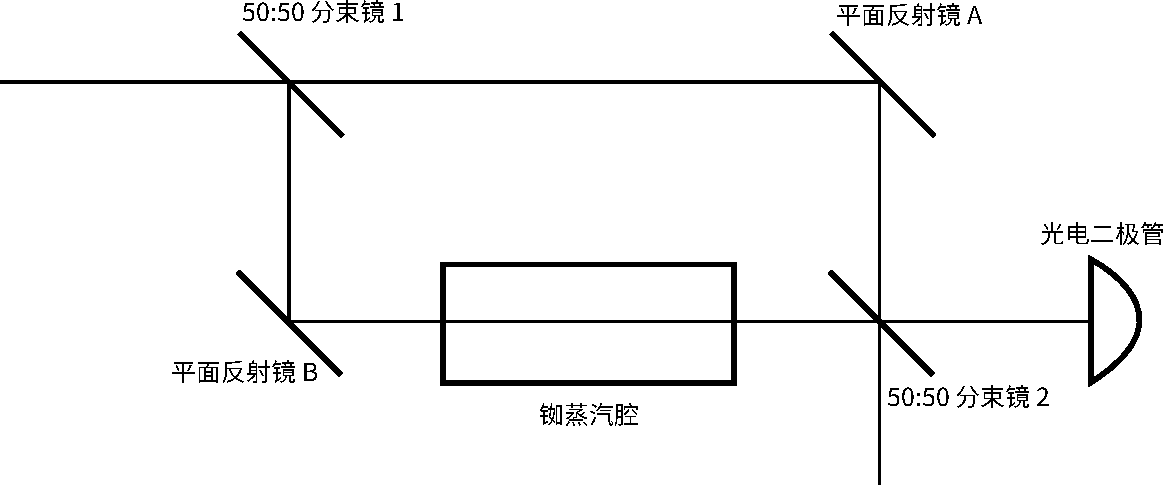
\includegraphics[width=.5\textwidth]{M-Z-Interferometer.pdf}
    \caption{M-Z干涉仪光路示意图}
    \label{M-Z}
\end{figure}

为了得到干涉光的强度随着激光频率的定量变化关系,我们从无铷蒸汽腔的情况开始讨论. 设激光的频率为$\omega$,入射时电场分量的振幅为$\sqrt{2}E_0$(忽略空气、分光镜和反射镜对激光的衰减和吸收),A、B两路光束走过的距离(注意,不是光程)分别为$L_1$和$L_2$. 假设不存在铷蒸汽腔,则A、B两路光束的电场振幅(注意,不是光强,无论是分开还是重合,直接分开/叠加的都是振幅!)均为原来的一半,再次叠加时得到的电场分量为
\begin{align}
    E=\frac{E_0}{2}e^{i\frac{\omega}{c}L_1}+\frac{E_0}{2}e^{i\frac{\omega}{c}L_2}.
\end{align}
干涉光强与入射光强的比值为
\begin{align}
    \label{I/I_0-without-cell}
    \frac{I}{I_0}=\frac{\abs{E}^2}{E_0^2}=\frac{1}{2}\left[1+\cos\left(\frac{\omega}{c}\Delta L\right)\right],
\end{align}
其中$\Delta L=L_2-L_1$,如图\ref{OutputWithoutRbCell}.
\begin{figure}[h]
    \centering
    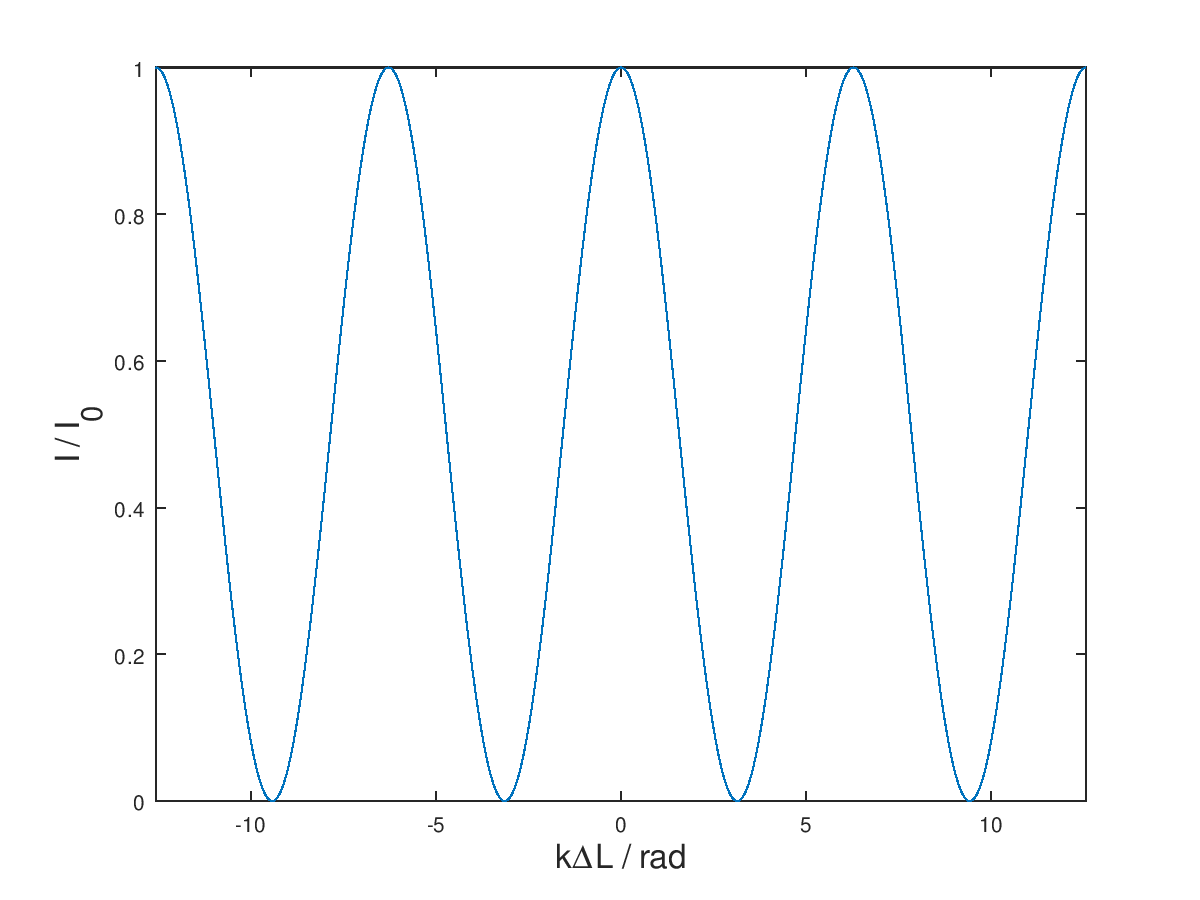
\includegraphics[width=.5\textwidth]{OutputWithoutCell.png}
    \caption{Photodiode output vs. $k\Delta L$, where $k=\omega/c=2\pi/\lambda$, for a perfect Mach-Zehnder interferometer with no rubidium cell, at fixed laser frequency.}
        \label{OutputWithoutRbCell}
\end{figure}

当存在长度为$\Delta z$的铷蒸汽腔,折射率为$n=n_0(1+i\kappa)$的铷蒸汽会给B路光束在原有相位上带来额外的相位差(这里指广义上的相位差,包含了衰减,为一复数):
\begin{align}
    e^{\frac{\omega}{c}(n-1)\Delta z}=e^{i\frac{\omega}{c}(n_0-1)\Delta z}e^{-\frac{\omega}{c}n_0\kappa\Delta z}=e^{i\delta}e^{-\tau},
\end{align}
其中铷蒸汽的吸收系数
\begin{align}
    \tau=\frac{\omega}{c}n_0\kappa\Delta z=\frac{\omega}{c}\frac{\pi Nfe^2}{m}\frac{\gamma/\omega_0}{\Delta\omega^2+\gamma^2}\Delta z\approx\frac{\pi Nfe^2}{cm\gamma}\frac{\gamma^2}{\Delta\omega^2+\gamma^2}\Delta z=\frac{\tau_0\gamma^2}{\Delta\omega^2+\gamma^2}\Delta z,
\end{align}
相移
\begin{align}
    \delta=\frac{\omega}{c}(n_0-1)\Delta z=-\frac{\omega}{c}\frac{\pi Nfe^2}{m}\frac{\Delta\omega/\omega_0}{\Delta\omega^2+\gamma^2}\Delta z\approx-\frac{\pi Nfe^2}{cm\gamma}\frac{\Delta\omega\gamma}{\Delta\omega^2+\gamma^2}\Delta z=-\frac{\tau_0\Delta\omega\gamma}{\Delta\omega^2+\gamma^2}\Delta z,
\end{align}
以上约等号成立的条件为$\omega\approx\omega_0$,其中
\begin{align}
    \tau_0=\frac{\pi Nfe^2}{cm\gamma}.
\end{align}
相移和吸收系数两者之间具有关系:
\begin{align}
    \delta=-\tau\frac{\Delta\omega}{\gamma}.
\end{align}
此时A、B两路光束再次叠加时得到的电场分量为
\begin{align}
    E=\frac{E_0}{2}e^{i\frac{\omega}{c}L_1}+\frac{E_0}{2}e^{-\tau}e^{i\frac{\omega}{c}L_2}e^{i\delta}.
\end{align}
干涉光强与入射光强的比值为
\begin{align}
    \frac{I}{I_0}=\frac{\abs{E}^2}{E_0^2}=\frac{1}{4}\left[1+e^{-2\tau}+e^{-\tau}\cos\left(\frac{\omega}{c}\Delta L+\delta\right)\right].
\end{align}
若$\tau=0$,$\delta=0$,上式即为无铷蒸汽腔的情况推出的式\eqref{I/I_0-without-cell}.

\section{书本问题求解}
\begin{prob}
    Consider the photodiode output from the interferometer without the rubidium cell. Figure \ref{OutputWithoutRbCell} shows the output at fixed laser frequency as a function of $\Delta L$. The maxima in this are referred to as "fringes", from their spatial structure (which you will see in the lab when you set up the interferometer). How small must $\Delta L$ be in order for the photodiode output to go through less than one fringe as the laser is scanned over the rubidium resonance line (call it $5$ GHz)? To get the best results, you should try to set up your interferometer with $\Delta L$ less than this.
\end{prob}
\begin{sol}
    为了使当激光扫过铷原子的共振频率范围($5$GHz)时光电探测器输出变化在一个fringe(即半个周期)以内,需要满足
    \begin{align}
        \Delta k\Delta L=\frac{2\pi\Delta\nu}{c}\Delta L=\frac{2\pi\times 5\times 10^9\text{Hz}}{3\times 10^8\text{m/s}}\Delta L\leq\pi,
    \end{align}
    即两条光路的光程差
    \begin{align}
        \Delta L\leq 3\times 10^{-2}\text{m}=3\text{cm}.
    \end{align}
\end{sol}

\begin{prob}
    Compute the photodiode output as a function of laser frequency around the rubidium resonance line, $I(\Delta\omega)/I_0$, for the set-up shown in Figure \ref{M-Z}. Assume the atoms in your cell are at rest (for ease of calculation) with some linewidth $\gamma$, so we can use the Lorentzian profile above for $\tau(\omega)$. Make three different plots of $I(\Delta\omega)/I_0$, one for each of three different values of the line center optical depth: $\tau_0=0.4$, $2$ and $20$. Make your plots over the range $-20\gamma<\Delta\omega<20\gamma$. Plot six curves on each plot, with values of $k\Delta L\mod(2\pi)$ equal to $j\pi/5$, with $j=0$ to $5$. The first and last of these correspond to the positions $A$ and $C$ in Figure \ref{OutputWithoutRbCell}. Label your plots. You will be trying to reproduce these curves in the lab. (Check your calculations by comparing with the one calculated curve in Figure )
    \begin{figure}[h]
        \centering
        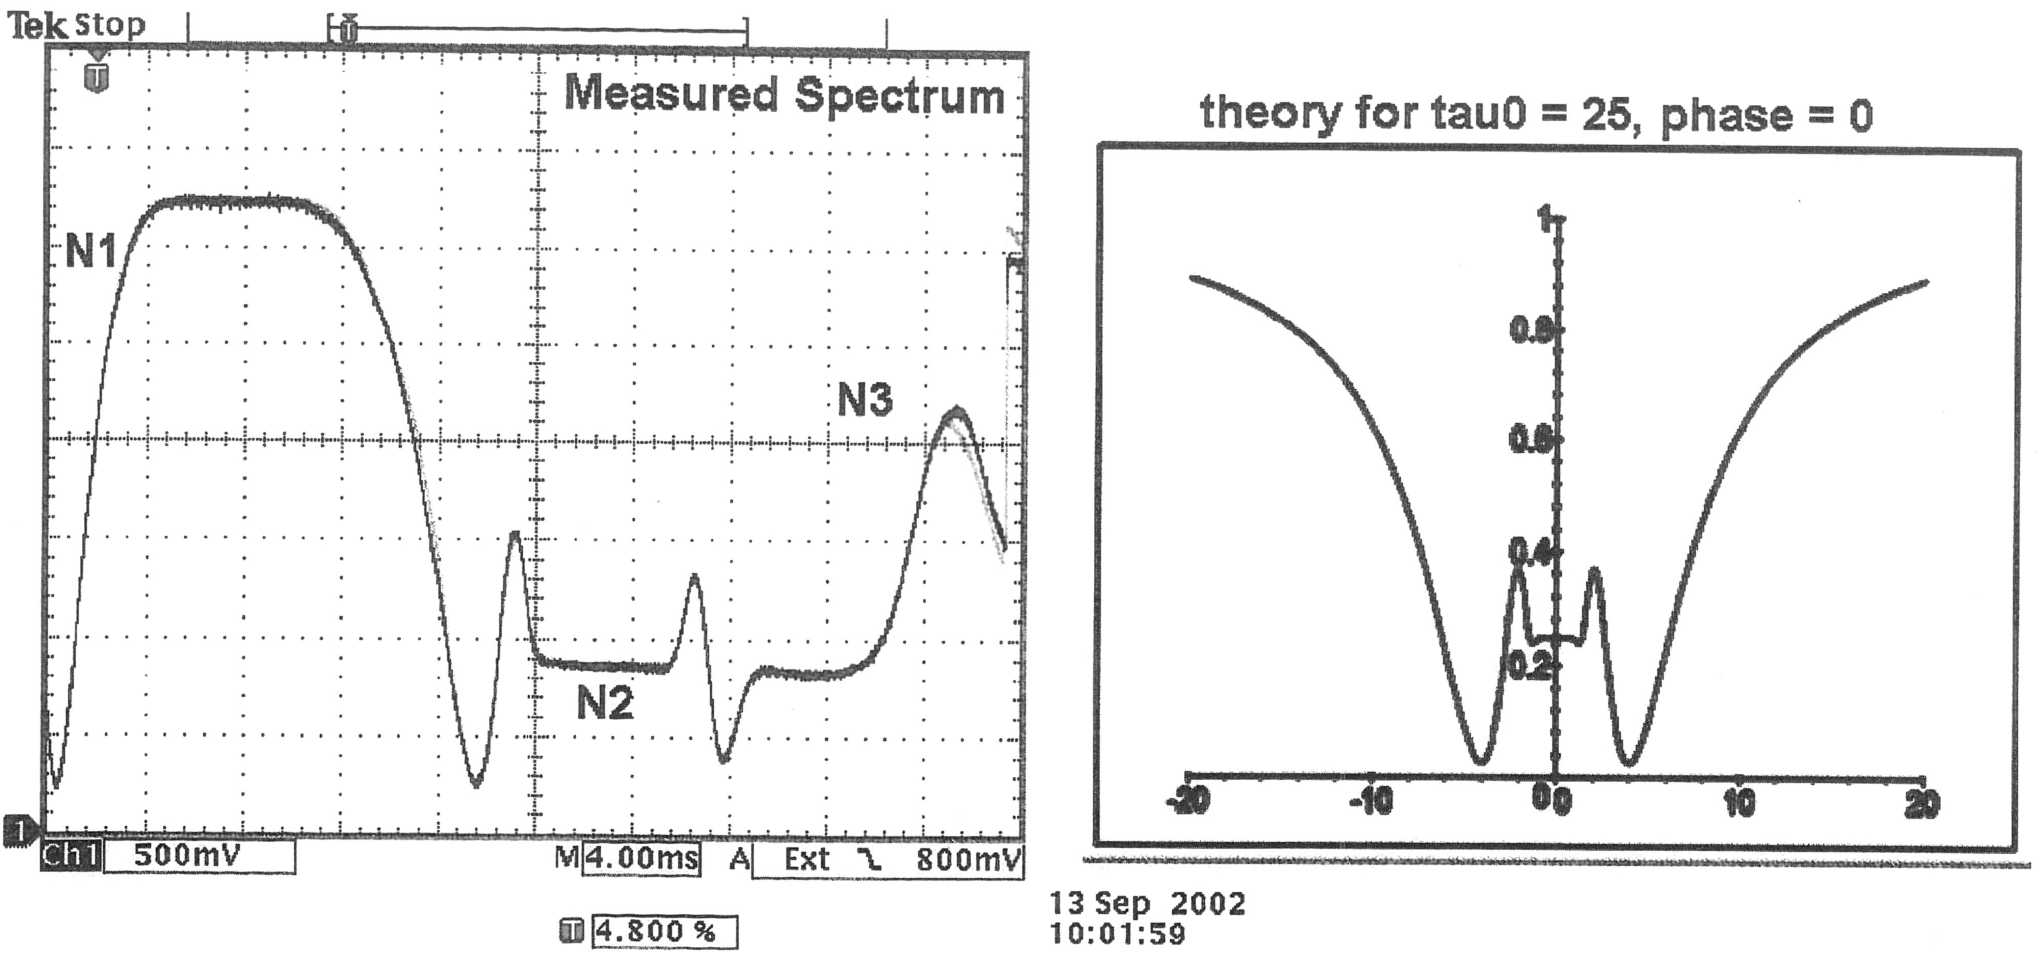
\includegraphics[width=.5\textwidth]{ComparisonOfMeasuredAndCalculatedSpectrum.png}
        \caption{A comparison of a measured spectrum (left) with a calculated spectrum (right). The plot shows $I(\Delta)/I_0$ versus $\Delta\omega/\gamma$. The calculation assumed $\tau=25$ at line center and $k\Delta L=0$. The measured spectrum is for the 85b line, but the adjacent 87b line complicates the right side of the spectrum (marked by N3). The center of the 85b line is at N2. The feature at N1 is an artifact of the laser scanning.}
    \end{figure}
\end{prob}
\begin{sol}
    当加入铷蒸汽腔,光电探测器的输出用频率可表为
    \begin{align}
        \frac{I(\Delta\omega)}{I_0}=\frac{1}{4}\left[1+e^{-2\tau}+2e^{-\tau}\cos\left(k\Delta L+\delta\right)\right].
    \end{align}
    其中
    \begin{align}
        \tau=&\frac{\tau_0\gamma^2}{\Delta\omega^2+\gamma^2},\\
        \delta=&-\tau\frac{\Delta\omega}{\gamma}.
    \end{align}
    按照题目要求分别代入$\tau_0=0.4,2,20$,分别绘制出$k\Delta L=0,\frac{\pi}{5},\frac{2\pi}{5},\cdots,\pi$对应的曲线,如图\ref{CalculatedSpectrum}.
    \begin{figure}[h]
        \centering
        \subfigure[$\tau_0=0.4$]{
        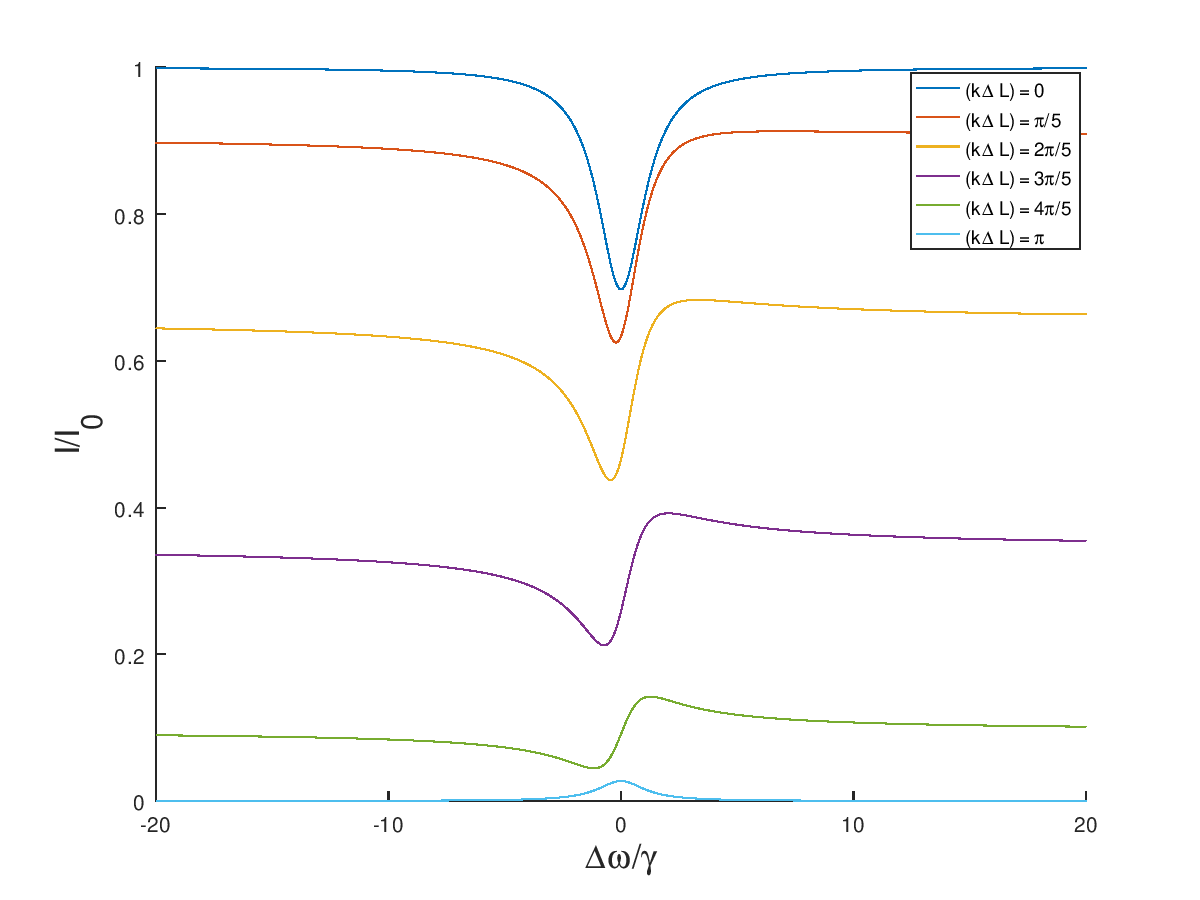
\includegraphics[width=0.45\textwidth]{Note-3-Problem-2-1.png}}
        \subfigure[$\tau_0=2$]{
        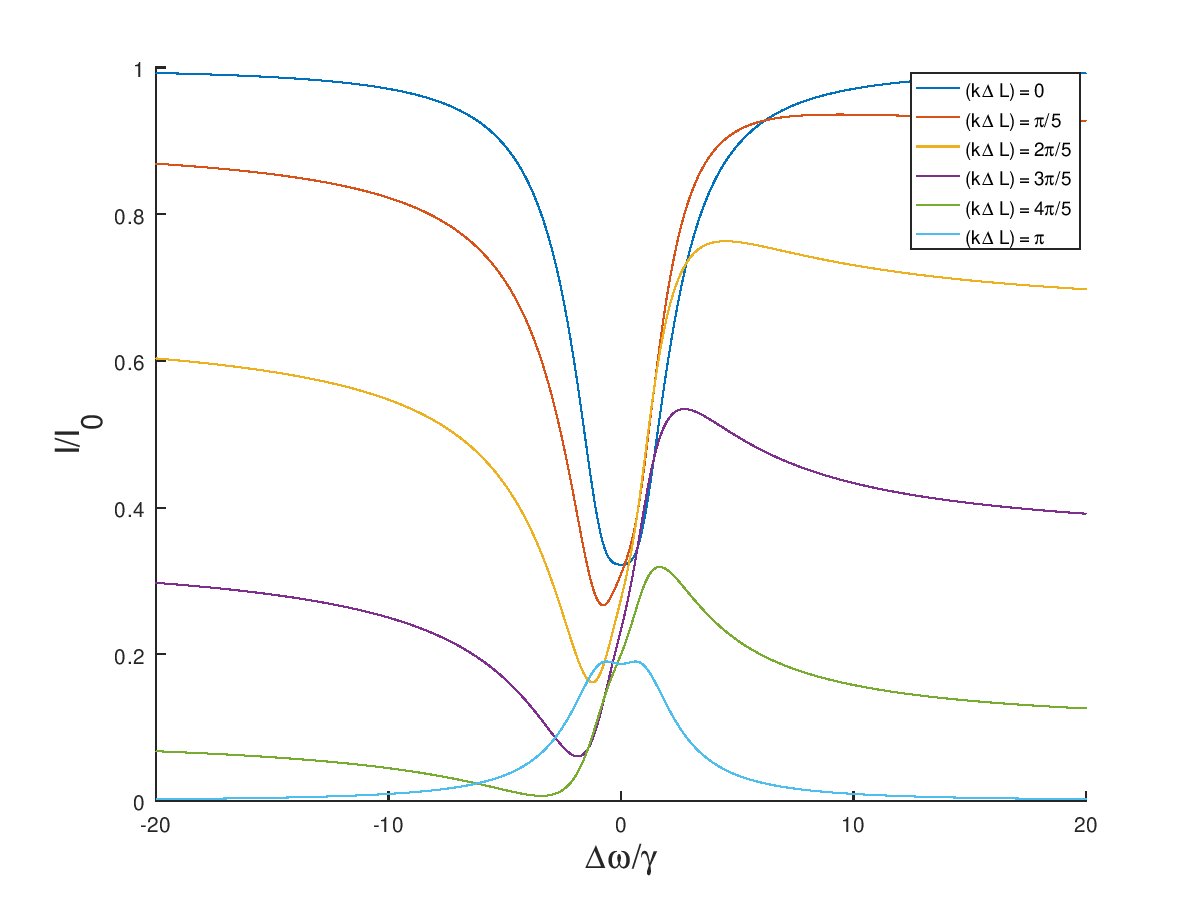
\includegraphics[width=0.45\textwidth]{Note-3-Problem-2-2.png}}
        \subfigure[$\tau_0=20$]{
        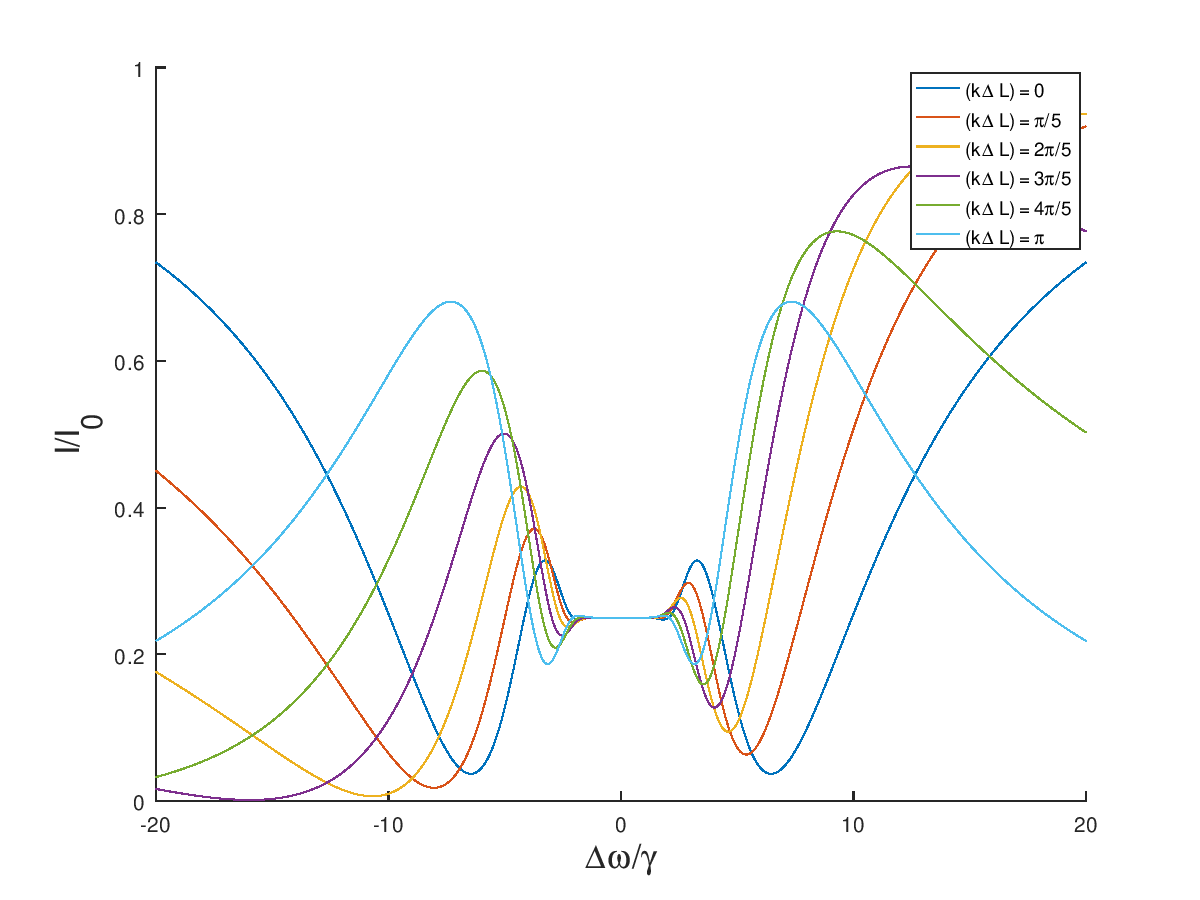
\includegraphics[width=0.45\textwidth]{Note-3-Problem-2-3.png}}
        \caption{计算所得:干涉光强随频率的变化关系}
        \label{CalculatedSpectrum}
    \end{figure}
\end{sol}
\end{document}
